% This is the Reed College LaTeX thesis template. Most of the work
% for the document class was done by Sam Noble (SN), as well as this
% template. Later comments etc. by Ben Salzberg (BTS). Additional
% restructuring and APA support by Jess Youngberg (JY).
% Your comments and suggestions are more than welcome; please email
% them to cus@reed.edu
%
% See http://web.reed.edu/cis/help/latex.html for help. There are a
% great bunch of help pages there, with notes on
% getting started, bibtex, etc. Go there and read it if you're not
% already familiar with LaTeX.
%
% Any line that starts with a percent symbol is a comment.
% They won't show up in the document, and are useful for notes
% to yourself and explaining commands.
% Commenting also removes a line from the document;
% very handy for troubleshooting problems. -BTS

% As far as I know, this follows the requirements laid out in
% the 2002-2003 Senior Handbook. Ask a librarian to check the
% document before binding. -SN

%%
%% Preamble
%%
% \documentclass{<something>} must begin each LaTeX document
\documentclass[12pt,twoside]{reedthesis}
% Packages are extensions to the basic LaTeX functions. Whatever you
% want to typeset, there is probably a package out there for it.
% Chemistry (chemtex), screenplays, you name it.
% Check out CTAN to see: http://www.ctan.org/
%%
\usepackage{graphicx,latexsym}
\usepackage{amsmath}
\usepackage{amssymb,amsthm}
\usepackage{longtable,booktabs,setspace}
\usepackage{chemarr} %% Useful for one reaction arrow, useless if you're not a chem major
\usepackage[hyphens]{url}
% Added by CII
\usepackage[hidelinks]{hyperref}
\usepackage{lmodern}
\usepackage{float}
\floatplacement{figure}{H}
% End of CII addition
\usepackage{rotating}

% Next line commented out by CII
%%% \usepackage{natbib}
% Comment out the natbib line above and uncomment the following two lines to use the new
% biblatex-chicago style, for Chicago A. Also make some changes at the end where the
% bibliography is included.
%\usepackage{biblatex-chicago}
%\bibliography{thesis}


% Added by CII (Thanks, Hadley!)
% Use ref for internal links
\renewcommand{\hyperref}[2][???]{\autoref{#1}}
\def\chapterautorefname{Chapter}
\def\sectionautorefname{Section}
\def\subsectionautorefname{Subsection}
% End of CII addition

% Added by CII
\usepackage{caption}
\captionsetup{width=5in}
% End of CII addition

% \usepackage{times} % other fonts are available like times, bookman, charter, palatino


% To pass between YAML and LaTeX the dollar signs are added by CII
\title{\textbf{\Huge{Numerical methods for stochastic volatility models: \\[20pt] Heston model}}}
\author{Fernando O. Teixeira}
% The month and year that you submit your FINAL draft TO THE LIBRARY (May or December)
\date{agosto 15, 2017}
\division{Applied Mathematics}
\advisor{Hugo Alexander de la Cruz Cancino}
%If you have two advisors for some reason, you can use the following
% Uncommented out by CII
% End of CII addition

%%% Remember to use the correct department!
\department{Mathematics}
% if you're writing a thesis in an interdisciplinary major,
% uncomment the line below and change the text as appropriate.
% check the Senior Handbook if unsure.
%\thedivisionof{The Established Interdisciplinary Committee for}
% if you want the approval page to say "Approved for the Committee",
% uncomment the next line
%\approvedforthe{Committee}

% Added by CII
%%% Copied from knitr
%% maxwidth is the original width if it's less than linewidth
%% otherwise use linewidth (to make sure the graphics do not exceed the margin)
\makeatletter
\def\maxwidth{ %
  \ifdim\Gin@nat@width>\linewidth
    \linewidth
  \else
    \Gin@nat@width
  \fi
}
\makeatother

\renewcommand{\contentsname}{Table of Contents}
% End of CII addition

\setlength{\parskip}{0pt}

% Added by CII

\providecommand{\tightlist}{%
  \setlength{\itemsep}{0pt}\setlength{\parskip}{0pt}}

\Acknowledgements{
I want to thank a few people. Any one who considers arithmetical methods
of producing random digits is, of course, in a state of sin. - John von
Neumann You get pseudo-order when you seek order; you only get a measure
of order and control when you embrace randomness. --- Nassim Nicholas
Taleb
}

\Dedication{
You can have a dedication here if you wish.
}

\Preface{

}

\Abstract{
The preface pretty much says it all. \par  Second paragraph of abstract
starts here.
}

	\usepackage{mathtools}
	\usepackage{cancel}
	\graphicspath{ {figure/} }
	\usepackage{enumitem}
% End of CII addition
%%
%% End Preamble
%%
%

\usepackage{amsthm}
\newtheorem{theorem}{Theorem}[section]
\newtheorem{lemma}{Lemma}[section]
\theoremstyle{definition}
\newtheorem{definition}{Definition}[section]
\newtheorem{corollary}{Corollary}[section]
\newtheorem{proposition}{Proposition}[section]
\theoremstyle{definition}
\newtheorem{example}{Example}[section]
\theoremstyle{remark}
\newtheorem*{remark}{Remark}
\begin{document}

% Everything below added by CII
      \maketitle
  
  \frontmatter % this stuff will be roman-numbered
  \pagestyle{empty} % this removes page numbers from the frontmatter
      \begin{acknowledgements}
      I want to thank a few people. Any one who considers arithmetical methods
      of producing random digits is, of course, in a state of sin. - John von
      Neumann You get pseudo-order when you seek order; you only get a measure
      of order and control when you embrace randomness. --- Nassim Nicholas
      Taleb
    \end{acknowledgements}
  
      \hypersetup{linkcolor=black}
    \setcounter{tocdepth}{2}
    \tableofcontents
  
      \listoftables
  
      \listoffigures
      \begin{abstract}
      The preface pretty much says it all. \par  Second paragraph of abstract
      starts here.
    \end{abstract}
      \begin{dedication}
      You can have a dedication here if you wish.
    \end{dedication}
  \mainmatter % here the regular arabic numbering starts
  \pagestyle{fancyplain} % turns page numbering back on

  \chapter{Introduction}\label{intro}
  
  The french mathematician Louis Bachelier was the trail-blazer that
  brought Brownian motion, previously restricted to the field of botanics
  where it was firstly observed, to the financial framework. He modeled
  the stock prices as a brownian motion with drift. In 1973, Black and
  Scholes {[}1{]} designed a model based on the geometric brownian motion
  to price options.
  
  Options are derivatives that give their bearers the rights to buy or
  sell a specific asset in a future date and with a predetermined price.
  They are, by design, affected by small variations in the underlying
  assets' components, for example, the variance.
  
  The Black-Scholes model was once the standard way of option pricing, but
  was replaced by more modern models that are now prevalent. One of the
  main drawbacks of the Black-Scholes model is the strong assumption that
  the stock returns' volatility is constant. Thus, the implied model's
  volatility results in a flat surface when plotted against the option's
  strike price and maturity. Real world implied volatility varies with the
  strike price and maturity, forming what is called the `volatility
  smile'.
  
  The Heston model is an extension of the Black-Scholes model that tackles
  this volatility issue replacing the constant volatility with a
  stochastic process. There are many models that stochastically model
  volatility, but the Heston has valuable characteristics suach as
  presenting an analytical solution to the option pricing and also having
  a computationally simple implementation when compared to more
  sophisticated competitors.
  
  This thesis is divided into five chapters, the first being this
  introduction. Following, we have a literature review that mainly
  addresses stochastic calculus, the Black-Scholes models and the Heston
  model. Thereafter we present the different Heston model known
  implementations and the implementation improvement we experiment.
  Chapter 4 brings the results of what was introduced in the previous
  chapter for different model calibrations.
  
  \chapter{Literature Review}\label{lt-review}
  
  This chapter presents the concepts of stochastic calculus, from the
  historic conception of how it first arose through the basic principles
  and applications in finance. We address with more care the classical
  Black-Scholes model and its limitations and the Heston model. This model
  is also well known, it brings the concept of stochastic volatility in
  it, which brings its results closer to reality.
  
  \section{Stochastic Calculus}\label{stochastic-calculus}
  
  Stochastic calculus arises from stochastic processes and allows the
  creation of a theory of integration where both the integrand and
  integrator terms are stochastic processes. Stochastic calculus was
  created by the Japanese mathematician Kiyosi Itô
  \footnote{There is another important stochastic integral, called the \textit{Stratonovich Integral} that unlike the Itô's integral, respects the conventional calculus chain rule. Also, the integral is evaluated at the interval's midpoint, instead of its left extreme. A Stratonovich integral can be expressed as an Itô integral and vice versa.}
  in the 1940s and 1950s and is used for modeling financial options and in
  another wide variety of fields {[}2{]}. In this chapter we present the
  historical contexts in which the tools and models used arise, but our
  focus is introducing the concepts and notations that will be further
  used in our work.
  
  \subsection{The Stochastic differential equation -
  SDE}\label{the-stochastic-differential-equation---sde}
  
  At first, before introducing stochastic differential equation, it is
  helpful to start with ordinary differential equation. Let \(x(t) = x_t\)
  denote the population at time \(t\) so that the change in the population
  at time \(t\) is given by the following deterministic differential
  equation:
  \begin{align}
  dx_t &= f(t, x_t)dt \\
  x(0) &= x_0 \nonumber
  \end{align}
  We now add a ``noise'' to this equation:
  \begin{align} \label{sde1}
  dx_t &= \overbrace{\underbrace{f(t, x_t)}_\text{drift}dt}^\text{deterministic} + \overbrace{\underbrace{g(t, x_t)}_\text{diffusion}dW_t}^\text{stochastic} \\
  x(0) &= x_0 \nonumber
  \end{align}
  This ``noise'' \(dW_t\) is a \emph{random} Wiener process time
  derivative (which will be clarified below) and \(X_0\) is our initial
  value.
  
  The \(g(t, x_t)\) part of the SDE is often referred as a \emph{diffusion
  process}. These processes generally have a continuous paths. Before
  moving on, we must carefully define what the term \emph{random}, means
  and the best way to begin doing so is to precisely define a probability
  space:
  \begin{definition}{(Probability Space)} A triple ($\Omega$, $\mathcal {U}$, $\mathcal {P}$) is called a \textit{probability space} provided $\Omega$ is any set, $\mathcal {U}$ is a $\sigma$-algebra of subsets of $\Omega$ and $\mathcal {P}$ is a probability measure on $\mathcal {U}$ .
  \end{definition}
  \subsection{Brownian Motion}\label{brownian-motion}
  
  The Brownian motion is the name given to the irregular motion observed
  in the motion of pollen particles suspended in fluid resulting from
  particle collision with atoms or molecules. It is named after Robert
  Brown, the first to have observed the movement in 1828. He noted two
  characteristic in the pollen movement {[}2{]}:
  \begin{itemize}
  \item
    the path of a given particle is very irregular, having a tangent at no
    point
  \item
    the motion of two distinct particles appear to be independent
  \end{itemize}
  The first quantitative works in brownian motion come from an interest in
  stock price fluctuation by Bachelier in 1900. Albert Einstein also
  leaned over the subject and in 1905 derived the transition density for
  Brownian motion from molecular-kinetic theory of heat {[}2,3{]}.
  
  In 1923, the Wiener process was coined in honor of Norbert Wiener
  mathematical proof of existence of the brownian motion and stating its
  properties.\footnote{More can be found on {[}4--6{]}.}
  \begin{definition}{(Wiener Process)} Given a probability space ($\Omega$, $\mathcal {U}$, $\mathcal {P}$), a stochastic process $W_t$ defined in this space is a \textit{wiener process} if it satisfies the following properties:
  \begin{itemize}
    \item  $W_{0}=0$
    
    \item The change in $W$, given by $\Delta W = W_{t+1}-W_{t}$, is normally distributed with mean zero and standard deviation $\sqrt{\Delta t}$, meaning that $\Delta W = \epsilon\sqrt{\Delta t}$, where $\epsilon$ is $N(0,1)$.
    
    \item If the increment $\Delta t_1$ does not overlap with the time increment $\Delta t_2$, then $\Delta W_1$ and $\Delta W_2$ are independent.
    
    \item The process is continuous, meaning that there are no jumps in the process.
    
    \item The process is a Markov process. This means that the conditional expectation of $W_{t+1}$ given its entire history is equal to the conditional expectation of $W_{t+1}$ given today's information. This can be written as: $E[W_{t+1}|W_1, ..., W_t] = E[W_{t+1}|W_t]$.
    
    \item Consider the time interval $[0,t]$ with $n$ equally spaced intervals given by $t_i = \frac{it}{n}$. Then the paths of the Brownian motion have unbounded variation, this means that they are not differentiable and go towards infinity as $n$ increases. The quadratic variation is given by $\sum_{i=1}^{n}{(Z_{t_i}-Z_{t_{i-1}})^2} \rightarrow t$, meaning that when $n$ increases it stays constant at $t$. 
  
  \end{itemize}
  \end{definition}
  \begin{figure}
  
  {\centering 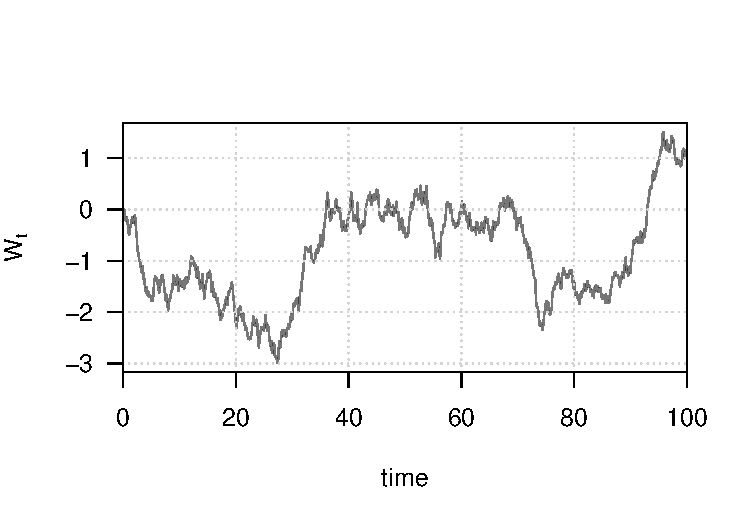
\includegraphics{thesis_files/figure-latex/wiener-1} 
  
  }
  
  \caption{A Wiener process trajectory path example \label{wiener}}\label{fig:wiener}
  \end{figure}
  \subsubsection{Correlated Brownian Motions}\label{corr}
  
  Two independent brownian motions that are correlated can describe a new
  process \(Z_t\). Let \(W_1\) and \(W_2\) be these two \emph{independent}
  Brownian motions and let \(-1 \leq \rho \leq 1\) be a given number. For
  \(0 \leq t \leq T\) define the new process \(Z_t\) as {[}2{]}:
  \begin{align}
  \label{eq:corr_brow}
  Z_t = \rho W_{1,t} + \sqrt{1-\rho^2}W_{2,t}
  \end{align}
  \noindent
  This equation is a linear combination of independent normals at each
  timestep \(t\), so \(Z_t\) is normally distributed. It is proven that
  \(Z\) is a Brownian motion and that \(Z\) and \(W_{1,t}\) are correlated
  {[}2{]}.
  
  \subsection{Itô's Integral}\label{itos-integral}
  
  Formally, the SDE presented in equation \ref{sde1} only exists because
  we can rewrite it in the form {[}5--10{]}:
  \begin{align} \label{sde1}
  x_t &= x_0 + \int_{0}^{t}{f(s, x_s)ds} + \int_{0}^{t}{g(s, x_s)dW_s}
  \end{align}
  \noindent
  for some \(f(s, x_s)\), \(g(s, x_s)\) and \(s \in [0,t]\).
  
  The Itô integral can, as the Riemann integral, be approximated by a
  finite sum. Also, it has a definition as a certain limit. Itô's lemma
  \ref{itolemma} plays the same role as the fundamental theorem of
  calculus in allowing to evaluate integrals. It is the formal definition
  and presents an extra term not encountered in the conventional calculus
  theorem that is due to the non-smoothness characteristics of Brownian
  motion paths. It is possible, though, to define the integral in a less
  rigorous way:
  \begin{align}
  Y_{\Delta t}(t) \approx \sum_{t_k < t}{g(t_k)\Delta W_k}
  \end{align}
  \noindent
  with the usual notions \(t_k = k\Delta t\), and
  \(\Delta W_k = W(t_{k+1})-W(t_k))\). If the limit exists, then the Ito
  integral is:
  \begin{align}
  Y(t)  = \lim\limits_{\Delta t \to 0} Y_{\Delta t}(t)
  \end{align}
  It is essential that the \emph{forward difference} is used rather than
  the backward difference, which would be \textbf{wrong}.
  \begin{theorem}[Itô's Lemma] \label{itolemma}
  Assume that $S_t$ has a stochastic differential given by:
  \begin{align}
  dS_t = \mu_t dt + \sigma_t dW_t 
  \end{align}
  \noindent
  for $\mu_t$, $\sigma_t$ and $t \in [0,T]$. Assume $u: \mathbb{R} \times [0, T] \rightarrow \mathbb{R}$ is continuous and that $\frac{\partial u}{\partial t}$, $\frac{\partial u}{\partial x}$, $\frac{\partial^2 u}{\partial x^2}$ exist and are continuous.
  
  $$Y_t := u(S_t, t)$$
  \noindent
  Then Y has the following stochastic differential:
  \begin{align} 
  \label{eq:ito}
  \begin{split}
      dY_t &= \frac{\partial u}{\partial t}dt + \frac{\partial u}{\partial x} dS_t + \frac{1}{2}\frac{\partial^2 u}{\partial x^2}\sigma_t^2 dt  \\[10pt] 
      &= \left( \frac{\partial u}{\partial t} + \mu_t \frac{\partial u}{\partial x} + \frac{1}{2}\frac{\partial^2 u}{\partial x^2}\sigma_t^2 \right) dt + \sigma_t \frac{\partial u}{\partial x} dW_t
  \end{split}
  \end{align}
  \noindent 
  where the argument of $u$, $\frac{\partial u}{\partial x}$ and $\frac{\partial^2 u}{\partial x^2}$ above is $\left( S_t, t \right)$ .
  \end{theorem}
  Equation \eqref{eq:ito} is the stochastic equivalent to the chain rule,
  also known as Itô's formula or Itô's chain rule. The proof to this
  theorem is based on the Taylor expansion of the function \(f(S_t, t)\)
  {[}5,7{]}. For practical uses you should write out a second-order Taylor
  expansion for the function to be analyzed and apply the
  \ref{tab:box-calc} multiplication table {[}2{]}.
  \begin{longtable}[t]{llr}
  \caption{\label{tab:box-calc}Box calculus}\\
  \toprule
    & $dt$ & $dW_t$\\
  \midrule
  $dt$ & 0 & 0\\
  $dW_t$ & 0 & $dt$\\
  \bottomrule
  \end{longtable}
  \begin{theorem}[Itô's Integral Properties]
  
  Let $f$, $g$ $\in$ $\mathcal{V}$ and let $0 \leq t_0 < u < T$. Then
  \begin{enumerate}[label=(\roman*)]
    \item $\int_{t_0}^{T}{f dB_t} = \int_{t_0}^{u}{f dB_t} + \int_{u}^{T}{f dB_t}$
    \item $\int_{t_0}^{T}{(\alpha f + \beta g) dB_t} = \alpha  \int_{t_0}^{T}{f dB_t} + \int_{t_0}^{T}{ \beta g dB_t}$
    \item $\mathbb{E}\left[ \int_{t_0}^{T}{fdB_t}\right] = 0 $
    \item $\mathbb {E} \left[\left(\int_{0}^{t}H_{s}\,dB_{s}\right)^{2}\right]=\mathbb {E} \left[\int _{0}^{t}H_{s}^{2}\,ds\right]$ (Isometry)
    \item $ \mathbb {E}\left[ \int_{t_0}^{T}{f dB_t \mid \mathcal{F}_{s}} \right] = \int_{t_0}^{s}{f dB_t}, \,\,\,\,\,\,\,\,\,\,\,\,\,\, for \,\, s < T.$  (Martingale\footnote{A martingale is a stochastic process with certain characteristics. The main one is that the expected value in time $t+1$ for $X$ is the $X$ value in $t$. This means there are no winning strategies when we are dealing with martingales (unlike when we play poker, for example). A Wiener process is a martingale.})
  \end{enumerate}
  \end{theorem}
  \section{Black-Scholes Model}\label{black-scholes-model}
  
  \subsection{Basics}\label{basics}
  
  The Black-Scholes (B-S) model arises from the need to price european
  options in the derivative markets. Derivatives are financial instruments
  traded in the market, stock exchange or over-the-counter (OTC) market,
  whose values depend on the values of an underlying asset. {[}1,11,12{]}
  \begin{itemize}
  \item
    A call option is a derivative that gives its bearer the right, but not
    the obligation, to purchase a specific asset by a fixed price before
    or on a given date.
  \item
    A put option is a derivative that gives its bearer the right, but not
    the obligation, to sell a specific asset by a fixed price before or on
    a given date.
  \end{itemize}
  The trading price of the option is called the option \emph{premium} and
  the asset from which the option derives is called the \emph{underlying
  asset}. This asset may be the interest rate, exchange rates, stock
  exchanges rates, commodities or stocks. The fixed price in contract in
  which the underlying asset might to be bought or sold is the
  \emph{strick price}. The option expiration date is called the
  \emph{maturity}. {[}1,12{]}
  
  There are two major different option types: the European and the
  American. The difference between these two is that the bearer of the
  first may exercise it only at the end of its life, at its maturity while
  the latter can be exercised at any given time until its maturity.
  {[}1,13{]}
  \begin{definition}{(Implicit volatility)} 
  Given all the option's parameters in a precification model and its market price, the option's volatility is called the \textit{implicit volatility}.
  \end{definition}
  \begin{definition}{(Intrinsic value)} 
  The intrinsic value of a call is the difference between the underlying asset price and the strike price. The put's intrinsic value operates the other way around, being the difference between the strike and the underling asset prices.
  \end{definition}
  \subsubsection{Geometric Brownian Motion}\label{gbm}
  
  A stochastic process \(S_t\) is a geometric brownian motion\footnote{There
    is an arithmetic brownian motion, whose equation is:
    \(dS_t = \mu dt + \sigma dB_t\). More information can be obatined
    about this process looking at {[}2{]}.} if its solution is described
  by the solution of the following stochastic differential equation
  {[}2,7,14{]}.
  \begin{align}
  dS_t = \mu S_t dt + \sigma S_t dW_t
  \end{align}
  \noindent
  for given constants \(\mu \in {\rm I\!R}\) and \(\sigma > 0\). Also, the
  assumed initial value is positive, \(S_0 >0\).
  
  This process\footnote{Also known as exponential brownian motion.}
  (Figure \ref{gbm}) is used quite often in finance to model the dynamics
  of some assets because of its properties. It has independent
  multiplicative increments and is the process used to price options in
  the Black-Scholes model {[}15{]}:
  \begin{align}
  S_t = S_0 \times exp{\left(\mu - \frac{\sigma^2}{2} \right) t + \sigma W_t}, \;\; t > 0
  \end{align}
  \begin{figure}
  
  {\centering 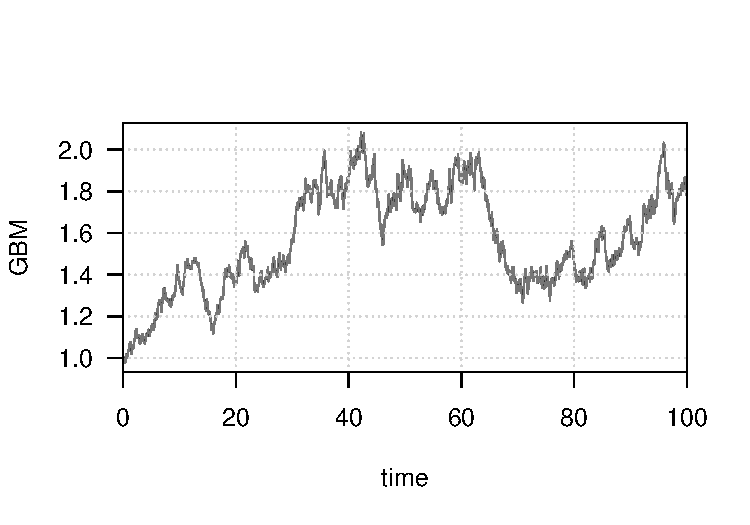
\includegraphics{thesis_files/figure-latex/gbm-1} 
  
  }
  
  \caption{A GBM trajectory path example \label{gbm}}\label{fig:gbm}
  \end{figure}
  \subsection{The model}\label{the-model}
  
  The Black-Scholes model that provides analytical solution to the price
  of a European call at time \(t\) can be described as follows
  {[}1,4,11{]}:
  \begin{align}
  C(S_{t},t)&=N(d_{1})S_{t}-N(d_{2})Ke^{-r(T-t)}\\[10pt]
  d_{1}&={\frac {1}{\sigma {\sqrt {T-t}}}}\left[\ln \left({\frac {S_{t}}{K}}\right)+\left(r+{\frac {\sigma ^{2}}{2}}\right)(T-t)\right]\\[10pt]
  d_{2}&=d_{1}-\sigma {\sqrt {T-t}}
  \end{align}
  \noindent
  Where:
  \begin{itemize}
  \tightlist
  \item
    \(S_{t}\) is the spot price of the underlying asset at time \(t\)
  \item
    \(r\) is the risk free rate (generally an annual
    rate)\footnote{Assumed to be constant. \label{teste}}
  \item
    \(\sigma\) is the volatility of returns of the underlying asset
    \footnote{See footnote 1.}
  \item
    \(N(\cdot )\) is the cumulative distribution function of the standard
    Gaussian distribution
  \item
    \(K\) is the strike price
  \item
    \(T-t\) is the time to maturity
  \end{itemize}
  \noindent
  Also, the stock price path is a Geometric Brownian Motion as previously
  stated, and is under the risk-neutral measure with the following
  dynamics {[}4,16{]}:
  \begin{align}
  dS_{t} = (r-q)S_td_t+\sigma S_t dW_t
  \end{align}
  \noindent
  Where \(dW_t\) is a Wiener process {[}1,16{]}, \(r\) is the risk free
  rate and \(q\) is the dividend
  yield\footnote{$r$ and $q$ are assumed to be constant.} and \(t\)
  denotes the current point in time.
  
  \subsection{Limitations}\label{limitations}
  
  Although the Black-Scholes is very popular and the \emph{de facto}
  standard in the market there are implications to the B-S model
  assumptions that affect the results and that are unrealistic. The main
  assumption that does not hold up is the deterministic (constant)
  volatility, that can more accurately be described as a stochastic
  process since we observe that small moves usually are followed by small
  moves and large moves by large moves. {[}4,11{]}
  
  Other assumptions that are critical to the B-S model and are not always
  observed in practice refer to the asset's continuity through time (no
  jumps), being allowed to perform continuous hedge without transactions
  costs and normal (Gaussian) returns.
  
  Most models focus on the volatility problem because transaction costs
  often translate to rises in volatility and fat-tails (abnormal) returns
  can be simulated by stochastic volatility and market or volatility
  jumps.
  
  \section{Stochastic Volatility
  models}\label{stochastic-volatility-models}
  
  Introducing stochastic volatility to models brings complexity, but
  enables modeling some features observed in reality that are crucial like
  the randomic market volatility effects, skewness (market returns are
  more realistically modeled) and volatility smile. This kind of model is
  applied highly succesfully in foreign exchange and credit markets.
  
  \subsection{Cox-Ingersoll-Ross model}\label{cir}
  
  The Cox-Ingersoll-Ross (CIR) model is a well-known short-rate model that
  describes the interest rate movements driven by one source of market
  risk. The dynamics are described as follows{[}17,18{]}:
  \begin{align}
  \label{eq:cir}
  dr_t &= k(\theta - r_t)dt + \sigma \sqrt{r_t} dB_t
  \end{align}
  \noindent
  Where, \(r_t\) is the short rate interest described by parameters \(k\)
  - the speed of mean reversion, \(\theta\) - the long-run mean variance
  and \(\sigma\) - the volatility of the variance process.
  
  This model has been widely used to describe the dynamics of the short
  rate interest because it has some fundamental features like intuitive
  parametrization, nonnegativity and pricing formulas. Besides, it takes
  account of anticipations, risk aversion, investment alternatives and
  preferences about consumption timing and allows for detailed predictions
  about how changes in a wide range of underlying variables affect the
  term structure{[}17{]}. Furthermore, this equation constitutes one of
  the two Heston model equations with the volatility taking the short rate
  interest place.
  
  \subsection{Heston Model}\label{heston-model}
  
  Heston model solves the deterministic volatility problems introducing
  the following equations, which represents the dynamics of the stock
  price and the variance processes under the risk-neutral measure
  {[}18,19{]}:
  \begin{align}
  \label{eq:heston}
  \begin{split}
  dS_t &= \mu S_t dt + \sqrt{V_t} S_t dW^*_t \\
  dV_t &= k(\theta - V_t)dt + \sigma \sqrt{V_t} dB_t
  \end{split}
  \end{align}
  The second equation, as described in Section \ref{cir}, is the CIR model
  equation. The first equation states the asset price process. \(\mu\) is
  the asset's rate of return, \(dW_{t,1}\) and \(dW_{t,2}\) are two
  correlated wiener processes with correlation coefficient of \(\rho\).
  Because, of the model specifications and what we presentend in section
  \ref{corr}, we can rewrite the first equation as in Broadie and Kaya
  {[}20{]}:
  \begin{align}
  \label{eq:heston2}
  \begin{split}
  dS_t &= \mu S_t dt + \rho \sqrt{V_t} dB_t + \sqrt{1 - \rho^2} \sqrt{V_t} S_t dW_t \\
  dV_t &= k(\theta - V_t)dt + \sigma \sqrt{V_t} dB_t
  \end{split}
  \end{align}
  \subsection{Other Models}\label{other-models}
  
  \subsubsection{Ornstein-Uhlenbeck}\label{ornstein-uhlenbeck}
  
  The Ornstein-Uhlenbeck is the earliest recorded SDE. Named after Leonard
  Ornstein and George Eugene Uhlenbeck, it is a stochastic process that
  describes the acceleration of a pollen particle in a liquid subject to
  bombardments by molecules {[}2{]}. As we can observe in equation
  @ref(ou\_eq), \(x_t\) represents the one dimension velocity of the
  particle, thus \(dx_t\) is the \emph{change} in velocity, in other
  words, its acceleration. The \(- \theta x_t\) component slows down the
  acceleration and is to be understood as frictional force. Besides, we
  add a noise \(W_t\) with intensity \(\sigma\) that models the random
  bombardment by the molecules.
  \begin{align} \label{ou_eq}
  &d x_t = - \theta x_t dt + \sigma d W_t \\
  \end{align}
  With \(\theta\) and \(\sigma\) being positive constants. Expressing in
  terms of \(x_t\) we get:
  \begin{align}
  x_t = e^{-\theta t} \times \left[ x_0  + \sigma \int_{t=0}^{T} e^{\theta t} d W_s \right] \,.
  \end{align}
  \subsubsection{Langevin}\label{langevin}
  
  The Langevin equation describes a system that consists of the molecular
  bombardment of a speck of dust on a water surface. We know that the
  intensity of the bombardement does not depend on the state variables
  {[}21{]}.
  \begin{align}
  m \frac{dv}{dt} = -\zeta v + \delta F (t) 
  \end{align}
  \(m\) is the mass of the particle, \(v\) it's velocity, \(-\zeta v\) is
  the frictional force, which is proportional to the velocity, and
  \(\delta F (t)\) is a \emph{fluctuating} force (random) to the
  frictional force.
  
  \section{Numerical Methods}\label{numerical-methods}
  
  Numerical methods are tools that are often applied to solve stochastic
  differential equations because most of these do not have explicit
  solution. This means that we are not able to solve these equations using
  symbolic computation. Although we are unable to find an analitical
  solution, when facing real problems, the approximation given by a
  numerical method is often sufficient. Alongside the analytical issue,
  the need to calculate the SDE's trajectory through time is the main
  reason why studying numerical methods is so important. An implementation
  of a numerical method is called a numerical algorithm.
  
  We will simulate sample paths of time discrete approximations
  implemented in the R programming language {[}22{]} that we base on a
  finite discretization of a time interval \([t_0, T]\). We shall generate
  approximate values of the sample path for each step contained in the
  discretized interval {[}21{]}.
  
  In the fixed step methods, the distance between two contiguous points is
  the distance
  \(d_i = t_i - t_{i-1} = \frac{T-t_0}{N} \;\;\; \forall i \mid 1 \leq i \leq N \in \mathbb{N}\).
  \(N\) being the time interval partition number.
  
  {[}21{]}
  
  The simulated sample paths can then be analysed by usual statistical
  methods to determine how good the approximation is and in what sense it
  is close to the exact solution. The state variables here are not
  discretized as in Kushner's Markov chain approach and the structure of
  the SDE as provided by the drift and diffusion coefficients is used in a
  natural way. An advantage of considerable practical importance of this
  approach is that the computational costs such as time and memory
  required increase only polynomially with the dimension of the problem.
  Variance reduction methods allow a considerable decrease in the required
  sample size.
  
  \subsection{Convergence ??}\label{convergence}
  
  \subsection{Euler-Maruyama}\label{euler-maruyama}
  
  \subsection{Milstein}\label{milstein}
  
  \subsection{Stability}\label{stability}
  
  {[}21{]} Most differential equations, deterministic or stochastic,
  cannot be solved explicitly. Nevertheless we can often deduce alot of
  useful information, usually qualitative, about the behaviour of their
  solutions from the functional form of their coefficients. Of particular
  interest in applications is the long term asymptotic behaviour and
  sensitivity of the solutions to small changes, for example measurement
  errors, in the initial values. From existence and uniqueness theory we
  know that the solutions of a differential equation are continuous in
  their initial values, at least over a finite time interval. Extending
  this idea to an infinite time interval leads to the concept of
  stability.
  
  \chapter{The Heston Model
  Implementation}\label{the-heston-model-implementation}
  
  \section{Characteristic Function}\label{characteristic-function}
  
  The Heston model characteristic function is firstly presented in the
  1993 Steven Heston's paper {[}18{]} and is described below {[}23{]}:
  \begin{align}
  f(S_t, V_t, t) = e^{A(T-t)+B(T-t)S_t + C(T-t)V_t + i \phi S_t}
  \end{align}
  If we let \(\tau = T-t\), then the explicit form of the Heston
  characteristic function is:
  \begin{align*}
  f(i \phi) &= e^{A(\tau)+B(\tau)S_t + C(\tau)V_t + i \phi S_t} \\
  A(\tau) &= r i \phi \tau + \frac{k \theta}{\sigma^2} \left[ - (\rho \sigma i \phi - k - M) \tau - 2 \ln\left(\frac{1-N e^{M \tau}}{1-N}\right) \right] \\
  B(\tau) &= 0 \\
  C(\tau) &= \frac{(e^{M \tau}-1)(\rho \sigma i \phi - k - M)}{\sigma^2 (1-N e^{M \tau})} \\
  \text{Where:} & \\
  M &= \sqrt{(\rho \sigma i \phi - k)^2 + \sigma^2 (i \phi + \phi^2)} \\
  N &= \frac{\rho \sigma i \phi - k - M}{\rho \sigma i \phi - k + M} \\
  \end{align*}
  This function is the driving force behind the following formula, that
  calculates the fair valur of a European call option at time \(t\), given
  a strike price \(K\), that expires at time \(T\) {[}23{]}:
  \begin{align} 
  \label{eq:cfheston}
  \begin{split}
  C = & \frac{1}{2} S(t) + \frac{e^{-r(T-t)}}{\pi}\int_{0}^{\infty}{\Re \left[ \frac{K^{-i \phi} f(i \phi + 1)}{i \phi} \right] d\phi} \\
  & -Ke^{-r(T-t)}\left( \frac{1}{2} + \frac{1}{\pi} \int_{0}^{\infty}{\Re \left[ \frac{K^{-i \phi} f(i \phi)}{i \phi} \right]}  d\phi \right)
  \end{split}
  \end{align}
  \section{Euler Scheme - Full
  Truncation}\label{euler-scheme---full-truncation}
  
  We present here the Euler Scheme - Full Truncation algorithm {[}20{]}
  along with some insights on how it was implemented in R. The Euler
  discretization brings approximation paths to stock prices and variance
  processes. If we set \(t_0 = 0 < t_1 < \dots < t_M = T\) as partitions
  of a time interval of \(M\) equal segments of lenght \(\delta t\), we
  have the following discretization for the stock price:
  \begin{align}
  S_{t+1} = S_t + rS_t + \sqrt{V_t} S_t Z_s
  \end{align}
  \noindent
  And for the variance process:
  \begin{align}
  V_{t+1} = V_t + k (\theta - V_t) + \sigma \sqrt{V_t} Z_v
  \end{align}
  \noindent
  \(Z_s\) being a standard normal random variable, i.e. \(N~(0,1)\), we
  set \(Z_t\) and \(Z_v\) as two independent standard normal random
  variables and \(Z_s\) and \(Z_v\) having correlation \(\rho\). This
  means we can write \(Z_s = \rho Z_v + \sqrt{1-\rho^2} Z_t\)
  
  The immediate observable problem in the proposed discretization scheme
  is that \(V\) can become negative with non-zero probability making the
  computation of \(\sqrt{V_t}\) impossible {[}24{]}. There are several
  proposed fixes that can be used, we chose the Full-Truncation (FT) and
  rewrite the equations as follows:
  \begin{align}
  S_{t+1} &= S_t + rS_t + \sqrt{V_{t}^{+}} S_t Z_s \\
  V_{t+1} &= V_t + k (\theta - V_{t}^{+}) + \sigma \sqrt{V_{t}^{+}} Z_v
  \end{align}
  \noindent
  Where we use the notation \(V_{t}^{+} = \max(V_{t}, 0)\).
  \begin{Shaded}
  \begin{Highlighting}[]
  \NormalTok{hestoneuler <-}\StringTok{ }\ControlFlowTok{function}\NormalTok{(S, X, r, v, theta, rho, k, sigma, }\DataTypeTok{t =} \DecValTok{0}\NormalTok{, }
                          \DataTypeTok{dt =} \OtherTok{NULL}\NormalTok{, }\DataTypeTok{tau =} \DecValTok{1}\NormalTok{, N, }\DataTypeTok{sensibility =} \DecValTok{15}\NormalTok{)\{}
  
      \KeywordTok{set.seed}\NormalTok{(}\DecValTok{1}\NormalTok{)}
  
      \ControlFlowTok{if}\NormalTok{(}\KeywordTok{is.null}\NormalTok{(dt))\{ dt <-}\StringTok{ }\NormalTok{(tau}\OperatorTok{-}\NormalTok{t)}\OperatorTok{/}\DecValTok{1000}\NormalTok{\}}
  
  \NormalTok{    ST <-}\StringTok{ }\OtherTok{NULL}
  \NormalTok{    aux <-}\StringTok{ }\OtherTok{NULL}
  \NormalTok{    sqrt_dt <-}\StringTok{ }\KeywordTok{sqrt}\NormalTok{(dt)}
  
      \ControlFlowTok{for}\NormalTok{(i }\ControlFlowTok{in} \KeywordTok{seq}\NormalTok{(t,tau,dt))\{}
          \CommentTok{# browser()}
  \NormalTok{        Zv <-}\StringTok{ }\KeywordTok{rnorm}\NormalTok{(N)}
  \NormalTok{        Zt <-}\StringTok{ }\KeywordTok{rnorm}\NormalTok{(N)}
  \NormalTok{        Zs <-}\StringTok{ }\NormalTok{rho }\OperatorTok{*}\StringTok{ }\NormalTok{Zv }\OperatorTok{+}\StringTok{ }\NormalTok{(}\KeywordTok{sqrt}\NormalTok{(}\DecValTok{1} \OperatorTok{-}\StringTok{ }\NormalTok{(rho}\OperatorTok{^}\DecValTok{2}\NormalTok{)) }\OperatorTok{*}\StringTok{ }\NormalTok{Zt)}
  
          \CommentTok{# v[v <= 0] = 0}
  
  \NormalTok{        aux <-}\StringTok{ }\NormalTok{v}
  \NormalTok{        aux[v }\OperatorTok{<}\StringTok{ }\DecValTok{0}\NormalTok{] <-}\StringTok{ }\DecValTok{0}
  \NormalTok{        sqrt_aux <-}\StringTok{ }\KeywordTok{sqrt}\NormalTok{(aux)}
  \NormalTok{        S <-}\StringTok{ }\NormalTok{S }\OperatorTok{*}\StringTok{ }\NormalTok{(}\DecValTok{1} \OperatorTok{+}\StringTok{ }\NormalTok{r }\OperatorTok{*}\StringTok{ }\NormalTok{dt }\OperatorTok{+}\StringTok{ }\NormalTok{sqrt_aux }\OperatorTok{*}\StringTok{ }\NormalTok{Zs }\OperatorTok{*}\StringTok{ }\NormalTok{sqrt_dt)}
  \NormalTok{        S[S }\OperatorTok{<=}\StringTok{ }\DecValTok{0}\NormalTok{] =}\StringTok{ }\DecValTok{0}
  
  \NormalTok{        v <-}\StringTok{ }\NormalTok{v }\OperatorTok{+}\StringTok{ }\NormalTok{k }\OperatorTok{*}\StringTok{ }\NormalTok{dt }\OperatorTok{*}\StringTok{ }\NormalTok{(theta }\OperatorTok{-}\StringTok{ }\NormalTok{aux) }\OperatorTok{+}\StringTok{ }
  \StringTok{          }\NormalTok{sigma }\OperatorTok{*}\StringTok{ }\NormalTok{sqrt_aux }\OperatorTok{*}\StringTok{ }\NormalTok{Zv }\OperatorTok{*}\StringTok{ }\NormalTok{sqrt_dt}
  
  \NormalTok{        ST <-}\StringTok{ }\KeywordTok{rbind}\NormalTok{(ST,S)}
  \NormalTok{    \}}
  
      \KeywordTok{rm}\NormalTok{(aux, v, Zv, Zt, Zs, S)}
  
  \NormalTok{    ST <-}\StringTok{ }\KeywordTok{as.matrix}\NormalTok{(ST, }\DataTypeTok{ncol=}\NormalTok{N)}
      \CommentTok{# matplot(graf, type = 'l')}
      \CommentTok{# abline(h=X, lwd=2, col='red')}
  \NormalTok{    media <-}\StringTok{ }\KeywordTok{c}\NormalTok{()}
  
      \ControlFlowTok{for}\NormalTok{ (j }\ControlFlowTok{in}\NormalTok{ (X}\OperatorTok{-}\NormalTok{sensibility)}\OperatorTok{:}\NormalTok{(X}\OperatorTok{+}\NormalTok{sensibility))\{}
  
  \NormalTok{        Result <-}\StringTok{ }\NormalTok{ST[}\KeywordTok{nrow}\NormalTok{(ST),] }\OperatorTok{-}\StringTok{ }\NormalTok{j}
  \NormalTok{        Result[Result }\OperatorTok{<=}\StringTok{ }\DecValTok{0}\NormalTok{] <-}\StringTok{ }\DecValTok{0}
  \NormalTok{        media <-}\KeywordTok{c}\NormalTok{(media, }\KeywordTok{mean}\NormalTok{(Result))}
  
  \NormalTok{    \}}
  
  \NormalTok{    media <-}\StringTok{ }\NormalTok{media }\OperatorTok{*}\StringTok{ }\KeywordTok{exp}\NormalTok{(}\OperatorTok{-}\NormalTok{r}\OperatorTok{*}\NormalTok{tau)}
      \CommentTok{# plot(media, ylab = "Call price", xlab = "Strike price")}
  
  \NormalTok{    Result <-}\StringTok{ }\NormalTok{ST[}\KeywordTok{nrow}\NormalTok{(ST),] }\OperatorTok{-}\StringTok{ }\NormalTok{X}
  \NormalTok{    Result[Result }\OperatorTok{<=}\StringTok{ }\DecValTok{0}\NormalTok{] =}\StringTok{ }\DecValTok{0}
  \NormalTok{    call =}\StringTok{ }\KeywordTok{mean}\NormalTok{(}\KeywordTok{exp}\NormalTok{(}\OperatorTok{-}\NormalTok{r}\OperatorTok{*}\NormalTok{tau)}\OperatorTok{*}\NormalTok{Result)}
  
  \NormalTok{    lista =}\StringTok{ }\KeywordTok{list}\NormalTok{(}\StringTok{'call'}\NormalTok{ =}\StringTok{ }\NormalTok{call, }\StringTok{'Result'}\NormalTok{ =}\StringTok{ }\NormalTok{Result, }
                   \StringTok{'Spot'}\NormalTok{ =}\StringTok{ }\NormalTok{ST, }\StringTok{'sensib'}\NormalTok{ =}\StringTok{ }\NormalTok{media)}
      \KeywordTok{return}\NormalTok{(lista)}
  \NormalTok{\}}
  \end{Highlighting}
  \end{Shaded}
  \section{Kahl-Jackel}\label{kahl-jackel}
  \begin{Shaded}
  \begin{Highlighting}[]
  \NormalTok{Hestoncallkj <-}\StringTok{ }\ControlFlowTok{function}\NormalTok{(S, X, r, q, v, theta, rho, k, sigma, }
                           \DataTypeTok{t =} \DecValTok{0}\NormalTok{, }\DataTypeTok{dt =} \OtherTok{NULL}\NormalTok{, }\DataTypeTok{tau =} \DecValTok{1}\NormalTok{, N, }
                           \DataTypeTok{sensibility =} \DecValTok{15}\NormalTok{)\{}
  
      \ControlFlowTok{if}\NormalTok{(}\KeywordTok{is.null}\NormalTok{(dt))\{ dt <-}\StringTok{ }\NormalTok{(T}\OperatorTok{-}\NormalTok{t)}\OperatorTok{/}\DecValTok{1000}\NormalTok{\}}
  
  \NormalTok{    v <-}\StringTok{ }\KeywordTok{rep}\NormalTok{(v,N)}
  \NormalTok{    theta<-}\StringTok{ }\KeywordTok{rep}\NormalTok{(theta,N)}
  \NormalTok{    graf <-}\StringTok{ }\OtherTok{NULL}
  \NormalTok{    S <-}\StringTok{ }\KeywordTok{log}\NormalTok{(S)}
  
      \ControlFlowTok{for}\NormalTok{(i }\ControlFlowTok{in} \KeywordTok{seq}\NormalTok{(t,tau,dt))\{}
       \CommentTok{# browser()}
  \NormalTok{    Zv <-}\StringTok{ }\KeywordTok{rnorm}\NormalTok{(N)}
  \NormalTok{    Zt <-}\StringTok{ }\KeywordTok{rnorm}\NormalTok{(N)}
  \NormalTok{    Zs <-}\StringTok{ }\NormalTok{rho }\OperatorTok{*}\StringTok{ }\NormalTok{Zv }\OperatorTok{+}\StringTok{ }\KeywordTok{sqrt}\NormalTok{(}\DecValTok{1} \OperatorTok{-}\StringTok{ }\NormalTok{rho}\OperatorTok{^}\DecValTok{2}\NormalTok{) }\OperatorTok{*}\StringTok{ }\NormalTok{Zt}
  
  \NormalTok{    vt <-}\StringTok{ }\NormalTok{(v }\OperatorTok{+}\StringTok{ }\NormalTok{k }\OperatorTok{*}\StringTok{ }\NormalTok{theta }\OperatorTok{*}\StringTok{ }\NormalTok{dt }\OperatorTok{+}\StringTok{ }\NormalTok{sigma }\OperatorTok{*}\StringTok{ }\KeywordTok{sqrt}\NormalTok{(v) }\OperatorTok{*}\StringTok{ }\NormalTok{Zv }\OperatorTok{*}\StringTok{ }\KeywordTok{sqrt}\NormalTok{(dt) }\OperatorTok{+}
  \StringTok{              }\NormalTok{(}\DecValTok{1}\OperatorTok{/}\DecValTok{4}\NormalTok{) }\OperatorTok{*}\StringTok{ }\NormalTok{sigma}\OperatorTok{^}\DecValTok{2} \OperatorTok{*}\StringTok{ }\NormalTok{dt }\OperatorTok{*}\StringTok{ }\NormalTok{((Zv)}\OperatorTok{^}\DecValTok{2} \OperatorTok{-}\StringTok{ }\DecValTok{1}\NormalTok{))}\OperatorTok{/}\NormalTok{(}\DecValTok{1} \OperatorTok{+}\StringTok{ }\NormalTok{k }\OperatorTok{*}\StringTok{ }\NormalTok{dt)}
  
      \CommentTok{# print(vt)}
  
      \CommentTok{# if(!length(vt[vt <= 0]) == 0 & length(vt[vt <= 0]) >= 1)\{}
      \CommentTok{#     # browser()}
  \NormalTok{    vt[vt }\OperatorTok{<=}\StringTok{ }\DecValTok{0}\NormalTok{] <-}\StringTok{ }\NormalTok{v[vt }\OperatorTok{<=}\StringTok{ }\DecValTok{0}\NormalTok{] }\OperatorTok{+}\StringTok{ }\NormalTok{k }\OperatorTok{*}\StringTok{ }\NormalTok{dt }\OperatorTok{*}\StringTok{ }\NormalTok{(theta[vt }\OperatorTok{<=}\StringTok{ }\DecValTok{0}\NormalTok{] }\OperatorTok{-}\StringTok{ }
  \StringTok{                    }\KeywordTok{pmax}\NormalTok{(v[vt }\OperatorTok{<=}\StringTok{ }\DecValTok{0}\NormalTok{],}\DecValTok{0}\NormalTok{)) }\OperatorTok{+}\StringTok{ }\NormalTok{sigma }\OperatorTok{*}\StringTok{ }
  \StringTok{                    }\KeywordTok{sqrt}\NormalTok{(}\KeywordTok{pmax}\NormalTok{(v[vt }\OperatorTok{<=}\StringTok{ }\DecValTok{0}\NormalTok{],}\DecValTok{0}\NormalTok{)) }\OperatorTok{*}\StringTok{ }\NormalTok{Zv[vt }\OperatorTok{<=}\StringTok{ }\DecValTok{0}\NormalTok{] }\OperatorTok{*}\StringTok{ }\KeywordTok{sqrt}\NormalTok{(dt)}
  \NormalTok{    v <-}\StringTok{ }\NormalTok{vt}
  \NormalTok{    v[v}\OperatorTok{<=}\DecValTok{0}\NormalTok{] <-}\StringTok{ }\DecValTok{0}
  
      \CommentTok{# \}}
  
  \NormalTok{    S <-}\StringTok{ }\NormalTok{S }\OperatorTok{+}\StringTok{ }\NormalTok{(r }\OperatorTok{-}\StringTok{ }\NormalTok{(v}\OperatorTok{+}\NormalTok{vt)}\OperatorTok{/}\DecValTok{4}\NormalTok{) }\OperatorTok{*}\StringTok{ }\NormalTok{dt }\OperatorTok{+}\StringTok{ }\NormalTok{rho }\OperatorTok{*}\StringTok{ }\KeywordTok{sqrt}\NormalTok{(}\KeywordTok{pmax}\NormalTok{(v,}\DecValTok{0}\NormalTok{)) }\OperatorTok{*}\StringTok{ }
  \StringTok{          }\NormalTok{Zv }\OperatorTok{*}\StringTok{ }\KeywordTok{sqrt}\NormalTok{(dt) }\OperatorTok{+}
  \StringTok{          }\NormalTok{(}\DecValTok{1}\OperatorTok{/}\DecValTok{2}\NormalTok{) }\OperatorTok{*}\StringTok{ }\NormalTok{(}\KeywordTok{sqrt}\NormalTok{(}\KeywordTok{pmax}\NormalTok{(v,}\DecValTok{0}\NormalTok{)) }\OperatorTok{+}\StringTok{ }\KeywordTok{sqrt}\NormalTok{(}\KeywordTok{pmax}\NormalTok{(vt,}\DecValTok{0}\NormalTok{))) }\OperatorTok{*}\StringTok{ }
  \StringTok{          }\NormalTok{(Zs }\OperatorTok{+}\StringTok{ }\NormalTok{rho }\OperatorTok{*}\StringTok{ }\NormalTok{Zv) }\OperatorTok{*}\StringTok{ }
  \StringTok{          }\KeywordTok{sqrt}\NormalTok{(dt) }\OperatorTok{+}
  \StringTok{          }\NormalTok{((rho }\OperatorTok{*}\StringTok{ }\NormalTok{sigma }\OperatorTok{*}\StringTok{ }\NormalTok{dt)}\OperatorTok{/}\DecValTok{2}\NormalTok{) }\OperatorTok{*}\StringTok{ }\NormalTok{((Zv)}\OperatorTok{^}\DecValTok{2} \OperatorTok{-}\StringTok{ }\DecValTok{1}\NormalTok{)}
  
  \NormalTok{    S[S }\OperatorTok{<=}\StringTok{ }\DecValTok{0}\NormalTok{] =}\StringTok{ }\DecValTok{0}
  \NormalTok{    graf <-}\StringTok{ }\KeywordTok{rbind}\NormalTok{(graf,S)}
  
  \NormalTok{    \}}
  
       \CommentTok{# browser()}
  
  \NormalTok{    graf <-}\StringTok{ }\KeywordTok{as.matrix}\NormalTok{(graf, }\DataTypeTok{ncol=}\NormalTok{N)}
  \NormalTok{    ST <-}\StringTok{ }\NormalTok{graf}
      \CommentTok{# matplot(graf, type = 'l')}
      \CommentTok{# abline(h=log(X), lwd=2, col='red')}
  
  \NormalTok{    media <-}\StringTok{ }\KeywordTok{c}\NormalTok{()}
  
      \CommentTok{# browser()}
  
      \ControlFlowTok{for}\NormalTok{ (j }\ControlFlowTok{in}\NormalTok{ (X}\OperatorTok{-}\NormalTok{sensibility)}\OperatorTok{:}\NormalTok{(X}\OperatorTok{+}\NormalTok{sensibility))\{}
  
  \NormalTok{        Result <-}\StringTok{ }\KeywordTok{exp}\NormalTok{(ST[}\KeywordTok{nrow}\NormalTok{(ST),]) }\OperatorTok{-}\StringTok{ }\NormalTok{j}
  \NormalTok{        Result[Result }\OperatorTok{<=}\StringTok{ }\DecValTok{0}\NormalTok{] <-}\StringTok{ }\DecValTok{0}
  \NormalTok{        media <-}\KeywordTok{c}\NormalTok{(media, }\KeywordTok{mean}\NormalTok{(Result))}
  
  \NormalTok{    \}}
  
  \NormalTok{    media <-}\StringTok{ }\NormalTok{media }\OperatorTok{*}\StringTok{ }\KeywordTok{exp}\NormalTok{(}\OperatorTok{-}\NormalTok{r}\OperatorTok{*}\NormalTok{tau)}
  
      \CommentTok{# browser()}
  
  \NormalTok{    Result <-}\StringTok{ }\KeywordTok{exp}\NormalTok{(ST[}\KeywordTok{nrow}\NormalTok{(ST),]) }\OperatorTok{-}\StringTok{ }\NormalTok{X}
  \NormalTok{    Result[Result }\OperatorTok{<=}\StringTok{ }\DecValTok{0}\NormalTok{] =}\StringTok{ }\DecValTok{0}
  \NormalTok{    call =}\StringTok{ }\KeywordTok{mean}\NormalTok{(}\KeywordTok{exp}\NormalTok{(}\OperatorTok{-}\NormalTok{r}\OperatorTok{*}\NormalTok{tau)}\OperatorTok{*}\NormalTok{Result)}
  
  \NormalTok{    lista =}\StringTok{ }\KeywordTok{list}\NormalTok{(}\StringTok{'call'}\NormalTok{ =}\StringTok{ }\NormalTok{call, }\StringTok{'Result'}\NormalTok{ =}\StringTok{ }\NormalTok{Result, }
                   \StringTok{'Spot'}\NormalTok{ =}\StringTok{ }\NormalTok{graf, }\StringTok{'sensib'}\NormalTok{ =}\StringTok{ }\NormalTok{media)}
      \KeywordTok{return}\NormalTok{(lista)}
  
  \NormalTok{\}}
  \end{Highlighting}
  \end{Shaded}
  \section{Exact Algorithm}\label{exact-algorithm}
  \begin{Shaded}
  \begin{Highlighting}[]
  \NormalTok{hestonea <-}\StringTok{ }\ControlFlowTok{function}\NormalTok{(S, X, r, v, theta, rho, k, sigma, }\DataTypeTok{t =} \DecValTok{0}\NormalTok{, }
                       \DataTypeTok{dt =} \OtherTok{NULL}\NormalTok{, }\DataTypeTok{tau =} \DecValTok{1}\NormalTok{, N, }\DataTypeTok{sensibility =} \DecValTok{15}\NormalTok{)\{}
  
      \ControlFlowTok{if}\NormalTok{(}\KeywordTok{is.null}\NormalTok{(dt))\{ dt <-}\StringTok{ }\NormalTok{(tau}\OperatorTok{-}\NormalTok{t)}\OperatorTok{/}\DecValTok{1000}\NormalTok{\}}
  
  \NormalTok{    ST <-}\StringTok{ }\OtherTok{NULL}
  
  \NormalTok{    d <-}\StringTok{ }\NormalTok{(}\DecValTok{4} \OperatorTok{*}\StringTok{ }\NormalTok{k }\OperatorTok{*}\StringTok{ }\NormalTok{theta)}\OperatorTok{/}\NormalTok{(sigma)}\OperatorTok{^}\DecValTok{2}
  \NormalTok{    c0 <-}\StringTok{ }\NormalTok{(sigma}\OperatorTok{^}\DecValTok{2} \OperatorTok{*}\StringTok{ }\NormalTok{(}\DecValTok{1} \OperatorTok{-}\StringTok{ }\KeywordTok{exp}\NormalTok{(}\OperatorTok{-}\NormalTok{k}\OperatorTok{*}\NormalTok{dt)))}\OperatorTok{/}\NormalTok{(}\DecValTok{4}\OperatorTok{*}\NormalTok{k)}
  
      \CommentTok{# browser()}
  
      \ControlFlowTok{for}\NormalTok{(i }\ControlFlowTok{in} \KeywordTok{seq}\NormalTok{(t,tau,dt))\{}
  
          \CommentTok{# sampling V}
  \NormalTok{        lambda <-}\StringTok{ }\NormalTok{(}\DecValTok{4}\OperatorTok{*}\NormalTok{k}\OperatorTok{*}\KeywordTok{exp}\NormalTok{(}\OperatorTok{-}\NormalTok{k}\OperatorTok{*}\NormalTok{dt)}\OperatorTok{*}\NormalTok{v)}\OperatorTok{/}\NormalTok{(sigma}\OperatorTok{^}\DecValTok{2} \OperatorTok{*}\StringTok{ }\NormalTok{(}\DecValTok{1}\OperatorTok{-}\KeywordTok{exp}\NormalTok{(}\OperatorTok{-}\NormalTok{k}\OperatorTok{*}\NormalTok{dt)))}
  \NormalTok{        vt <-}\StringTok{ }\NormalTok{c0 }\OperatorTok{*}\StringTok{ }\KeywordTok{rchisq}\NormalTok{(}\DataTypeTok{n =}\NormalTok{ N, }\DataTypeTok{df =}\NormalTok{ d, }\DataTypeTok{ncp =}\NormalTok{ lambda)}
  
          \CommentTok{# Sampling int\{V\}}
  \NormalTok{        int_v <-}\StringTok{ }\NormalTok{dt }\OperatorTok{*}\StringTok{ }\NormalTok{((}\DecValTok{1}\OperatorTok{/}\DecValTok{2}\NormalTok{) }\OperatorTok{*}\StringTok{ }\NormalTok{v }\OperatorTok{+}\StringTok{ }\NormalTok{(}\DecValTok{1}\OperatorTok{/}\DecValTok{2}\NormalTok{) }\OperatorTok{*}\StringTok{ }\NormalTok{vt)}
  
          \CommentTok{# Sampling int\{v\}dw}
  \NormalTok{        int_vdw <-}\StringTok{ }\NormalTok{(}\DecValTok{1}\OperatorTok{/}\NormalTok{sigma) }\OperatorTok{*}\StringTok{ }\NormalTok{(vt }\OperatorTok{-}\StringTok{ }\NormalTok{v }\OperatorTok{-}\StringTok{ }\NormalTok{k }\OperatorTok{*}\StringTok{ }\NormalTok{theta }\OperatorTok{*}\StringTok{ }\NormalTok{dt }\OperatorTok{+}\StringTok{ }\NormalTok{k  }\OperatorTok{*}\StringTok{ }\NormalTok{int_v)}
  
          \CommentTok{# Sampling S}
  \NormalTok{        m <-}\StringTok{ }\KeywordTok{log}\NormalTok{(S) }\OperatorTok{+}\StringTok{ }\NormalTok{(r }\OperatorTok{*}\StringTok{ }\NormalTok{dt }\OperatorTok{-}\StringTok{ }\NormalTok{(}\DecValTok{1}\OperatorTok{/}\DecValTok{2}\NormalTok{) }\OperatorTok{*}\StringTok{ }\NormalTok{int_v }\OperatorTok{+}\StringTok{ }\NormalTok{rho }\OperatorTok{*}\StringTok{ }\NormalTok{int_vdw)}
  \NormalTok{        std <-}\StringTok{ }\KeywordTok{sqrt}\NormalTok{((}\DecValTok{1} \OperatorTok{-}\StringTok{ }\NormalTok{rho}\OperatorTok{^}\DecValTok{2}\NormalTok{)) }\OperatorTok{*}\StringTok{ }\KeywordTok{sqrt}\NormalTok{(int_v)}
  \NormalTok{        S <-}\StringTok{ }\KeywordTok{exp}\NormalTok{(m }\OperatorTok{+}\StringTok{ }\NormalTok{std }\OperatorTok{*}\StringTok{ }\KeywordTok{rnorm}\NormalTok{(N))}
  \NormalTok{        v <-}\StringTok{ }\NormalTok{vt}
  \NormalTok{        ST <-}\StringTok{ }\KeywordTok{rbind}\NormalTok{(ST,S)}
  \NormalTok{    \}}
  
  \NormalTok{    ST <-}\StringTok{ }\KeywordTok{as.matrix}\NormalTok{(ST, }\DataTypeTok{ncol=}\NormalTok{N)}
      \CommentTok{# matplot(graf, type = 'l')}
      \CommentTok{# abline(h=X, lwd=2, col='red')}
  \NormalTok{    media <-}\StringTok{ }\KeywordTok{c}\NormalTok{()}
  
      \ControlFlowTok{for}\NormalTok{ (j }\ControlFlowTok{in}\NormalTok{ (X}\OperatorTok{-}\NormalTok{sensibility)}\OperatorTok{:}\NormalTok{(X}\OperatorTok{+}\NormalTok{sensibility))\{}
  
  \NormalTok{        Result <-}\StringTok{ }\NormalTok{ST[}\KeywordTok{nrow}\NormalTok{(ST),] }\OperatorTok{-}\StringTok{ }\NormalTok{j}
  \NormalTok{        Result[Result }\OperatorTok{<=}\StringTok{ }\DecValTok{0}\NormalTok{] <-}\StringTok{ }\DecValTok{0}
  \NormalTok{        media <-}\KeywordTok{c}\NormalTok{(media, }\KeywordTok{mean}\NormalTok{(Result))}
  
  \NormalTok{    \}}
  
  \NormalTok{    media <-}\StringTok{ }\NormalTok{media }\OperatorTok{*}\StringTok{ }\KeywordTok{exp}\NormalTok{(}\OperatorTok{-}\NormalTok{r}\OperatorTok{*}\NormalTok{tau)}
      \CommentTok{# plot(media, ylab = "Call price", xlab = "Strike price")}
  
  \NormalTok{    Result <-}\StringTok{ }\NormalTok{ST[}\KeywordTok{nrow}\NormalTok{(ST),] }\OperatorTok{-}\StringTok{ }\NormalTok{X}
  \NormalTok{    Result[Result }\OperatorTok{<=}\StringTok{ }\DecValTok{0}\NormalTok{] =}\StringTok{ }\DecValTok{0}
  \NormalTok{    call =}\StringTok{ }\KeywordTok{mean}\NormalTok{(}\KeywordTok{exp}\NormalTok{(}\OperatorTok{-}\NormalTok{r}\OperatorTok{*}\NormalTok{tau)}\OperatorTok{*}\NormalTok{Result)}
  
  \NormalTok{    lista =}\StringTok{ }\KeywordTok{list}\NormalTok{(}\StringTok{'call'}\NormalTok{ =}\StringTok{ }\NormalTok{call, }\StringTok{'Result'}\NormalTok{ =}\StringTok{ }\NormalTok{Result, }
                   \StringTok{'Spot'}\NormalTok{ =}\StringTok{ }\NormalTok{ST, }\StringTok{'sensib'}\NormalTok{ =}\StringTok{ }\NormalTok{media)}
      \KeywordTok{return}\NormalTok{(lista)}
  \NormalTok{\}}
  \end{Highlighting}
  \end{Shaded}
  \clearpage
  \begin{Shaded}
  \begin{Highlighting}[]
  \KeywordTok{require}\NormalTok{(NMOF)}
  \KeywordTok{setwd}\NormalTok{(}\StringTok{"../rnmethods"}\NormalTok{)}
  \KeywordTok{source}\NormalTok{(}\StringTok{"../rnmethods/R/euler_heston.R"}\NormalTok{)}
  \end{Highlighting}
  \end{Shaded}
  \chapter{Results}\label{results}
  
  \chapter{Conclusion}\label{conclusion}
  
  If we don't want Conclusion to have a chapter number next to it, we can
  add the \texttt{\{-\}} attribute.
  
  \textbf{More info}
  
  And here's some other random info: the first paragraph after a chapter
  title or section head \emph{shouldn't be} indented, because indents are
  to tell the reader that you're starting a new paragraph. Since that's
  obvious after a chapter or section title, proper typesetting doesn't add
  an indent there.
  
  \appendix
  
  \chapter{The First Appendix}\label{the-first-appendix}
  
  This first appendix includes all of the R chunks of code that were
  hidden throughout the document (using the \texttt{include\ =\ FALSE}
  chunk tag) to help with readibility and/or setup.
  
  \textbf{In the main Rmd file}
  \begin{Shaded}
  \begin{Highlighting}[]
  \CommentTok{# This chunk ensures that the thesisdown package is}
  \CommentTok{# installed and loaded. This thesisdown package includes}
  \CommentTok{# the template files for the thesis.}
  \ControlFlowTok{if}\NormalTok{(}\OperatorTok{!}\KeywordTok{require}\NormalTok{(devtools))}
    \KeywordTok{install.packages}\NormalTok{(}\StringTok{"devtools"}\NormalTok{, }\DataTypeTok{repos =} \StringTok{"http://cran.rstudio.com"}\NormalTok{)}
  \ControlFlowTok{if}\NormalTok{(}\OperatorTok{!}\KeywordTok{require}\NormalTok{(thesisdown))}
  \NormalTok{  devtools}\OperatorTok{::}\KeywordTok{install_github}\NormalTok{(}\StringTok{"ismayc/thesisdown"}\NormalTok{)}
  \KeywordTok{library}\NormalTok{(thesisdown)}
  \end{Highlighting}
  \end{Shaded}
  \textbf{In Chapter \ref{ref-labels}:}
  \begin{Shaded}
  \begin{Highlighting}[]
  \CommentTok{# This chunk ensures that the thesisdown package is}
  \CommentTok{# installed and loaded. This thesisdown package includes}
  \CommentTok{# the template files for the thesis and also two functions}
  \CommentTok{# used for labeling and referencing}
  \ControlFlowTok{if}\NormalTok{(}\OperatorTok{!}\KeywordTok{require}\NormalTok{(devtools))}
    \KeywordTok{install.packages}\NormalTok{(}\StringTok{"devtools"}\NormalTok{, }\DataTypeTok{repos =} \StringTok{"http://cran.rstudio.com"}\NormalTok{)}
  \ControlFlowTok{if}\NormalTok{(}\OperatorTok{!}\KeywordTok{require}\NormalTok{(dplyr))}
      \KeywordTok{install.packages}\NormalTok{(}\StringTok{"dplyr"}\NormalTok{, }\DataTypeTok{repos =} \StringTok{"http://cran.rstudio.com"}\NormalTok{)}
  \ControlFlowTok{if}\NormalTok{(}\OperatorTok{!}\KeywordTok{require}\NormalTok{(ggplot2))}
      \KeywordTok{install.packages}\NormalTok{(}\StringTok{"ggplot2"}\NormalTok{, }\DataTypeTok{repos =} \StringTok{"http://cran.rstudio.com"}\NormalTok{)}
  \ControlFlowTok{if}\NormalTok{(}\OperatorTok{!}\KeywordTok{require}\NormalTok{(ggplot2))}
      \KeywordTok{install.packages}\NormalTok{(}\StringTok{"bookdown"}\NormalTok{, }\DataTypeTok{repos =} \StringTok{"http://cran.rstudio.com"}\NormalTok{)}
  \ControlFlowTok{if}\NormalTok{(}\OperatorTok{!}\KeywordTok{require}\NormalTok{(thesisdown))\{}
    \KeywordTok{library}\NormalTok{(devtools)}
  \NormalTok{  devtools}\OperatorTok{::}\KeywordTok{install_github}\NormalTok{(}\StringTok{"ismayc/thesisdown"}\NormalTok{)}
  \NormalTok{  \}}
  \KeywordTok{library}\NormalTok{(thesisdown)}
  \NormalTok{flights <-}\StringTok{ }\KeywordTok{read.csv}\NormalTok{(}\StringTok{"data/flights.csv"}\NormalTok{)}
  \end{Highlighting}
  \end{Shaded}
  \chapter{The Second Appendix, for
  Fun}\label{the-second-appendix-for-fun}
  
  \backmatter
  
  \chapter*{References}\label{references}
  \addcontentsline{toc}{chapter}{References}
  
  \noindent
  
  \setlength{\parindent}{-0.20in} \setlength{\leftskip}{0.20in}
  \setlength{\parskip}{8pt}
  
  \hypertarget{refs}{}
  \hypertarget{ref-black1973pricing}{}
  {[}1{]} F. Black, M. Scholes, The pricing of options and corporate
  liabilities, Journal of Political Economy. 81 (1973) 637--654.
  
  \hypertarget{ref-ubbo}{}
  {[}2{]} U.F. Wiersema, Brownian motion calculus, John Wiley \& Sons,
  2008.
  
  \hypertarget{ref-karatzas2012brownian}{}
  {[}3{]} I. Karatzas, S. Shreve, Brownian motion and stochastic calculus,
  Springer Science \& Business Media, 2012.
  
  \hypertarget{ref-helgadottir2016option}{}
  {[}4{]} A.D. Helgadóttir, L. Ionescu, Option pricing within the heston
  model, (2016).
  
  \hypertarget{ref-evans}{}
  {[}5{]} L.C. Evans, An introduction to stochastic differential
  equations, American Mathematical Soc., 2012.
  
  \hypertarget{ref-rosenthal}{}
  {[}6{]} J.S. Rosenthal, A first look at rigorous probability theory,
  World Scientific Publishing Co Inc, 2006.
  
  \hypertarget{ref-tong2012option}{}
  {[}7{]} Z. Tong, Option pricing with long memory stochastic volatility
  models, PhD thesis, Université d'Ottawa/University of Ottawa, 2012.
  
  \hypertarget{ref-steele2012stochastic}{}
  {[}8{]} J.M. Steele, Stochastic calculus and financial applications,
  Springer Science \& Business Media, 2012.
  
  \hypertarget{ref-ito1951}{}
  {[}9{]} K. Itō, On stochastic differential equations, American
  Mathematical Soc., 1951.
  
  \hypertarget{ref-ito1962}{}
  {[}10{]} K. Itô, The brownian motion and tensor fields on riemannian
  manifold, Proc. Int. Congr. Math., Stockholm. 2 (1962).
  
  \hypertarget{ref-yang2013valuing}{}
  {[}11{]} Y. Yang, Valuing a european option with the heston model,
  (2013).
  
  \hypertarget{ref-salomao2011precificaccao}{}
  {[}12{]} M. de F. Salomão, Precificação de opções financeiras: Um estudo
  sobre os modelos de black scholes e garch, (2011).
  
  \hypertarget{ref-merton1973theory}{}
  {[}13{]} R.C. Merton, Theory of rational option pricing, The Bell
  Journal of Economics and Management Science. (1973) 141--183.
  
  \hypertarget{ref-tsay2005analysis}{}
  {[}14{]} R.S. Tsay, Analysis of financial time series, John Wiley \&
  Sons, 2005.
  
  \hypertarget{ref-iacus2009simulation}{}
  {[}15{]} S.M. Iacus, Simulation and inference for stochastic
  differential equations: With r examples, Springer Science \& Business
  Media, 2009.
  
  \hypertarget{ref-nmof}{}
  {[}16{]} M. Gilli, D. Maringer, E. Schumann, Numerical methods and
  optimization in finance, Academic Press, Waltham, MA, USA, 2011.
  \url{http://nmof.net}.
  
  \hypertarget{ref-cox1985theory}{}
  {[}17{]} J.C. Cox, J.E. Ingersoll Jr, S.A. Ross, A theory of the term
  structure of interest rates, Econometrica: Journal of the Econometric
  Society. (1985) 385--407.
  
  \hypertarget{ref-heston1993closed}{}
  {[}18{]} S.L. Heston, A closed-form solution for options with stochastic
  volatility with applications to bond and currency options, Review of
  Financial Studies. 6 (1993) 327--343.
  
  \hypertarget{ref-gilli_numerical_2011}{}
  {[}19{]} M. Gilli, D. Maringer, E. Schumann, Numerical methods and
  optimization in finance, Academic Press, 2011.
  
  \hypertarget{ref-broadie2006exact}{}
  {[}20{]} M. Broadie, Ö. Kaya, Exact simulation of stochastic volatility
  and other affine jump diffusion processes, Operations Research. 54
  (2006) 217--231.
  
  \hypertarget{ref-kloeden1992}{}
  {[}21{]} P.E. Kloeden, E. Platen, Numerical solution of stochastic
  differential equations springer-verlag, 1992.
  
  \hypertarget{ref-rlang}{}
  {[}22{]} R Core Team, R: A language and environment for statistical
  computing, R Foundation for Statistical Computing, Vienna, Austria,
  2017. \url{https://www.R-project.org/}.
  
  \hypertarget{ref-dunn2014estimating}{}
  {[}23{]} R. Dunn, P. Hauser, T. Seibold, H. Gong, Estimating option
  prices with heston's stochastic volatility model, (2014).
  
  \hypertarget{ref-andersen2007efficient}{}
  {[}24{]} L.B. Andersen, Efficient simulation of the heston stochastic
  volatility model, (2007).


  % Index?

\end{document}
